% Created by tikzDevice version 0.12.3.1 on 2022-04-18 14:55:48
% !TEX encoding = UTF-8 Unicode
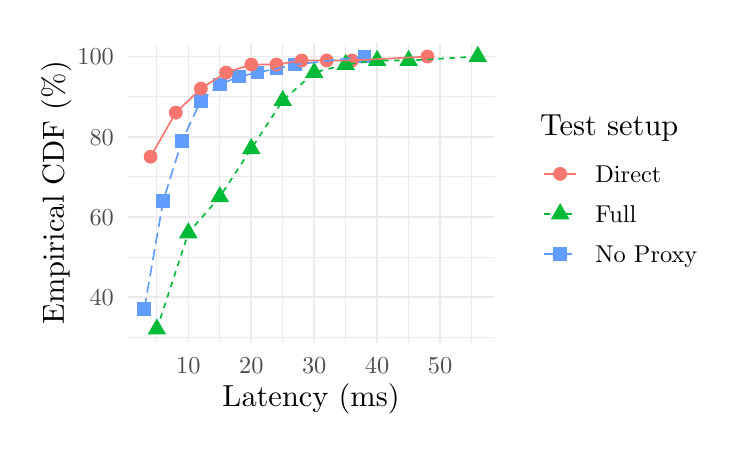
\begin{tikzpicture}[x=1pt,y=1pt]
\definecolor{fillColor}{RGB}{255,255,255}
\path[use as bounding box,fill=fillColor,fill opacity=0.00] (0,0) rectangle (252.94,144.54);
\begin{scope}
\path[clip] ( 36.11, 30.69) rectangle (168.69,139.04);
\definecolor{drawColor}{gray}{0.92}

\path[draw=drawColor,line width= 0.3pt,line join=round] ( 36.11, 32.71) --
	(168.69, 32.71);

\path[draw=drawColor,line width= 0.3pt,line join=round] ( 36.11, 61.69) --
	(168.69, 61.69);

\path[draw=drawColor,line width= 0.3pt,line join=round] ( 36.11, 90.66) --
	(168.69, 90.66);

\path[draw=drawColor,line width= 0.3pt,line join=round] ( 36.11,119.63) --
	(168.69,119.63);

\path[draw=drawColor,line width= 0.3pt,line join=round] ( 46.69, 30.69) --
	( 46.69,139.04);

\path[draw=drawColor,line width= 0.3pt,line join=round] ( 69.43, 30.69) --
	( 69.43,139.04);

\path[draw=drawColor,line width= 0.3pt,line join=round] ( 92.17, 30.69) --
	( 92.17,139.04);

\path[draw=drawColor,line width= 0.3pt,line join=round] (114.91, 30.69) --
	(114.91,139.04);

\path[draw=drawColor,line width= 0.3pt,line join=round] (137.65, 30.69) --
	(137.65,139.04);

\path[draw=drawColor,line width= 0.3pt,line join=round] (160.39, 30.69) --
	(160.39,139.04);

\path[draw=drawColor,line width= 0.6pt,line join=round] ( 36.11, 47.20) --
	(168.69, 47.20);

\path[draw=drawColor,line width= 0.6pt,line join=round] ( 36.11, 76.17) --
	(168.69, 76.17);

\path[draw=drawColor,line width= 0.6pt,line join=round] ( 36.11,105.14) --
	(168.69,105.14);

\path[draw=drawColor,line width= 0.6pt,line join=round] ( 36.11,134.11) --
	(168.69,134.11);

\path[draw=drawColor,line width= 0.6pt,line join=round] ( 58.06, 30.69) --
	( 58.06,139.04);

\path[draw=drawColor,line width= 0.6pt,line join=round] ( 80.80, 30.69) --
	( 80.80,139.04);

\path[draw=drawColor,line width= 0.6pt,line join=round] (103.54, 30.69) --
	(103.54,139.04);

\path[draw=drawColor,line width= 0.6pt,line join=round] (126.28, 30.69) --
	(126.28,139.04);

\path[draw=drawColor,line width= 0.6pt,line join=round] (149.02, 30.69) --
	(149.02,139.04);
\definecolor{fillColor}{RGB}{97,156,255}

\path[fill=fillColor] ( 39.64, 40.36) --
	( 44.63, 40.36) --
	( 44.63, 45.35) --
	( 39.64, 45.35) --
	cycle;

\path[fill=fillColor] ( 46.46, 79.47) --
	( 51.46, 79.47) --
	( 51.46, 84.46) --
	( 46.46, 84.46) --
	cycle;

\path[fill=fillColor] ( 53.28,101.20) --
	( 58.28,101.20) --
	( 58.28,106.19) --
	( 53.28,106.19) --
	cycle;

\path[fill=fillColor] ( 60.11,115.68) --
	( 65.10,115.68) --
	( 65.10,120.68) --
	( 60.11,120.68) --
	cycle;

\path[fill=fillColor] ( 66.93,121.48) --
	( 71.92,121.48) --
	( 71.92,126.47) --
	( 66.93,126.47) --
	cycle;

\path[fill=fillColor] ( 73.75,124.37) --
	( 78.75,124.37) --
	( 78.75,129.37) --
	( 73.75,129.37) --
	cycle;

\path[fill=fillColor] ( 80.57,125.82) --
	( 85.57,125.82) --
	( 85.57,130.82) --
	( 80.57,130.82) --
	cycle;

\path[fill=fillColor] ( 87.39,127.27) --
	( 92.39,127.27) --
	( 92.39,132.27) --
	( 87.39,132.27) --
	cycle;

\path[fill=fillColor] ( 94.22,128.72) --
	( 99.21,128.72) --
	( 99.21,133.72) --
	( 94.22,133.72) --
	cycle;

\path[fill=fillColor] (119.23,131.62) --
	(124.23,131.62) --
	(124.23,136.61) --
	(119.23,136.61) --
	cycle;
\definecolor{fillColor}{RGB}{248,118,109}

\path[fill=fillColor] ( 44.41, 97.90) circle (  2.50);

\path[fill=fillColor] ( 53.51,113.83) circle (  2.50);

\path[fill=fillColor] ( 62.60,122.53) circle (  2.50);

\path[fill=fillColor] ( 71.70,128.32) circle (  2.50);

\path[fill=fillColor] ( 80.80,131.22) circle (  2.50);

\path[fill=fillColor] ( 89.89,131.22) circle (  2.50);

\path[fill=fillColor] ( 98.99,132.67) circle (  2.50);

\path[fill=fillColor] (108.08,132.67) circle (  2.50);

\path[fill=fillColor] (117.18,132.67) circle (  2.50);

\path[fill=fillColor] (144.47,134.11) circle (  2.50);
\definecolor{fillColor}{RGB}{0,186,56}

\path[fill=fillColor] ( 46.69, 39.50) --
	( 50.05, 33.67) --
	( 43.32, 33.67) --
	cycle;

\path[fill=fillColor] ( 58.06, 74.26) --
	( 61.42, 68.44) --
	( 54.69, 68.44) --
	cycle;

\path[fill=fillColor] ( 69.43, 87.30) --
	( 72.79, 81.47) --
	( 66.06, 81.47) --
	cycle;

\path[fill=fillColor] ( 80.80,104.68) --
	( 84.16, 98.86) --
	( 77.43, 98.86) --
	cycle;

\path[fill=fillColor] ( 92.17,122.06) --
	( 95.53,116.24) --
	( 88.80,116.24) --
	cycle;

\path[fill=fillColor] (103.54,132.20) --
	(106.90,126.38) --
	(100.17,126.38) --
	cycle;

\path[fill=fillColor] (114.91,135.10) --
	(118.27,129.28) --
	(111.54,129.28) --
	cycle;

\path[fill=fillColor] (126.28,136.55) --
	(129.64,130.72) --
	(122.91,130.72) --
	cycle;

\path[fill=fillColor] (137.65,136.55) --
	(141.01,130.72) --
	(134.28,130.72) --
	cycle;

\path[fill=fillColor] (162.66,138.00) --
	(166.02,132.17) --
	(159.30,132.17) --
	cycle;
\definecolor{drawColor}{RGB}{248,118,109}

\path[draw=drawColor,line width= 0.6pt,line join=round] ( 44.41, 97.90) --
	( 53.51,113.83) --
	( 62.60,122.53) --
	( 71.70,128.32) --
	( 80.80,131.22) --
	( 89.89,131.22) --
	( 98.99,132.67) --
	(108.08,132.67) --
	(117.18,132.67) --
	(144.47,134.11);
\definecolor{drawColor}{RGB}{0,186,56}

\path[draw=drawColor,line width= 0.6pt,dash pattern=on 2pt off 2pt ,line join=round] ( 46.69, 35.61) --
	( 58.06, 70.38) --
	( 69.43, 83.41) --
	( 80.80,100.80) --
	( 92.17,118.18) --
	(103.54,128.32) --
	(114.91,131.22) --
	(126.28,132.67) --
	(137.65,132.67) --
	(162.66,134.11);
\definecolor{drawColor}{RGB}{97,156,255}

\path[draw=drawColor,line width= 0.6pt,dash pattern=on 4pt off 2pt ,line join=round] ( 42.14, 42.85) --
	( 48.96, 81.97) --
	( 55.78,103.69) --
	( 62.60,118.18) --
	( 69.43,123.97) --
	( 76.25,126.87) --
	( 83.07,128.32) --
	( 89.89,129.77) --
	( 96.71,131.22) --
	(121.73,134.11);
\end{scope}
\begin{scope}
\path[clip] (  0.00,  0.00) rectangle (252.94,144.54);
\definecolor{drawColor}{gray}{0.30}

\node[text=drawColor,anchor=base east,inner sep=0pt, outer sep=0pt, scale=  0.88] at ( 31.16, 44.17) {40};

\node[text=drawColor,anchor=base east,inner sep=0pt, outer sep=0pt, scale=  0.88] at ( 31.16, 73.14) {60};

\node[text=drawColor,anchor=base east,inner sep=0pt, outer sep=0pt, scale=  0.88] at ( 31.16,102.11) {80};

\node[text=drawColor,anchor=base east,inner sep=0pt, outer sep=0pt, scale=  0.88] at ( 31.16,131.08) {100};
\end{scope}
\begin{scope}
\path[clip] (  0.00,  0.00) rectangle (252.94,144.54);
\definecolor{drawColor}{gray}{0.30}

\node[text=drawColor,anchor=base,inner sep=0pt, outer sep=0pt, scale=  0.88] at ( 58.06, 19.68) {10};

\node[text=drawColor,anchor=base,inner sep=0pt, outer sep=0pt, scale=  0.88] at ( 80.80, 19.68) {20};

\node[text=drawColor,anchor=base,inner sep=0pt, outer sep=0pt, scale=  0.88] at (103.54, 19.68) {30};

\node[text=drawColor,anchor=base,inner sep=0pt, outer sep=0pt, scale=  0.88] at (126.28, 19.68) {40};

\node[text=drawColor,anchor=base,inner sep=0pt, outer sep=0pt, scale=  0.88] at (149.02, 19.68) {50};
\end{scope}
\begin{scope}
\path[clip] (  0.00,  0.00) rectangle (252.94,144.54);
\definecolor{drawColor}{RGB}{0,0,0}

\node[text=drawColor,anchor=base,inner sep=0pt, outer sep=0pt, scale=  1.10] at (102.40,  7.64) {Latency (ms)};
\end{scope}
\begin{scope}
\path[clip] (  0.00,  0.00) rectangle (252.94,144.54);
\definecolor{drawColor}{RGB}{0,0,0}

\node[text=drawColor,rotate= 90.00,anchor=base,inner sep=0pt, outer sep=0pt, scale=  1.10] at ( 13.08, 84.86) {Empirical CDF (\%)};
\end{scope}
\begin{scope}
\path[clip] (  0.00,  0.00) rectangle (252.94,144.54);
\definecolor{drawColor}{RGB}{0,0,0}

\node[text=drawColor,anchor=base west,inner sep=0pt, outer sep=0pt, scale=  1.10] at (185.19,105.51) {Test setup};
\end{scope}
\begin{scope}
\path[clip] (  0.00,  0.00) rectangle (252.94,144.54);
\definecolor{fillColor}{RGB}{248,118,109}

\path[fill=fillColor] (192.41, 91.71) circle (  2.50);
\end{scope}
\begin{scope}
\path[clip] (  0.00,  0.00) rectangle (252.94,144.54);
\definecolor{drawColor}{RGB}{248,118,109}

\path[draw=drawColor,line width= 0.6pt,line join=round] (186.63, 91.71) -- (198.20, 91.71);
\end{scope}
\begin{scope}
\path[clip] (  0.00,  0.00) rectangle (252.94,144.54);
\definecolor{fillColor}{RGB}{0,186,56}

\path[fill=fillColor] (192.41, 81.14) --
	(195.78, 75.31) --
	(189.05, 75.31) --
	cycle;
\end{scope}
\begin{scope}
\path[clip] (  0.00,  0.00) rectangle (252.94,144.54);
\definecolor{drawColor}{RGB}{0,186,56}

\path[draw=drawColor,line width= 0.6pt,dash pattern=on 2pt off 2pt ,line join=round] (186.63, 77.26) -- (198.20, 77.26);
\end{scope}
\begin{scope}
\path[clip] (  0.00,  0.00) rectangle (252.94,144.54);
\definecolor{fillColor}{RGB}{97,156,255}

\path[fill=fillColor] (189.92, 60.30) --
	(194.91, 60.30) --
	(194.91, 65.30) --
	(189.92, 65.30) --
	cycle;
\end{scope}
\begin{scope}
\path[clip] (  0.00,  0.00) rectangle (252.94,144.54);
\definecolor{drawColor}{RGB}{97,156,255}

\path[draw=drawColor,line width= 0.6pt,dash pattern=on 4pt off 2pt ,line join=round] (186.63, 62.80) -- (198.20, 62.80);
\end{scope}
\begin{scope}
\path[clip] (  0.00,  0.00) rectangle (252.94,144.54);
\definecolor{drawColor}{RGB}{0,0,0}

\node[text=drawColor,anchor=base west,inner sep=0pt, outer sep=0pt, scale=  0.88] at (205.14, 88.68) {Direct};
\end{scope}
\begin{scope}
\path[clip] (  0.00,  0.00) rectangle (252.94,144.54);
\definecolor{drawColor}{RGB}{0,0,0}

\node[text=drawColor,anchor=base west,inner sep=0pt, outer sep=0pt, scale=  0.88] at (205.14, 74.23) {Full};
\end{scope}
\begin{scope}
\path[clip] (  0.00,  0.00) rectangle (252.94,144.54);
\definecolor{drawColor}{RGB}{0,0,0}

\node[text=drawColor,anchor=base west,inner sep=0pt, outer sep=0pt, scale=  0.88] at (205.14, 59.77) {No Proxy};
\end{scope}
\end{tikzpicture}
